%!TEX root = ../thesis.tex

実環境への適用可能性を調査するため，自律走行競技会AI-Formula \cite{aiformula}における消失点ナビゲーションおよび障害物検出・停止タスクへ提案手法の応用を試みた．\Fig{fig:mobility}にAI-Formulaのモビリティを示す．モビリティには，ステレオカメラ，GNSS，IMUが搭載されている．\Fig{fig:aiformula_course}にAI-Formulaのコースを示す．コースは，白線や横断歩道などの情報があり，比較的平坦な地形となっている．本競技会では，実環境におけるリアルタイム認識と制御が要求される実践的な評価環境が提供されている．

\begin{figure}[H]
\centering
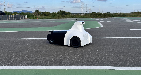
\includegraphics[width=1.0\linewidth]{images/pdf/ai-formula_mobility_resize.pdf}
\caption{AI-Formula mobility. (source: \cite{lang_sam_tracker})}
\label{fig:mobility}
\end{figure}

\begin{figure}[H]
\centering
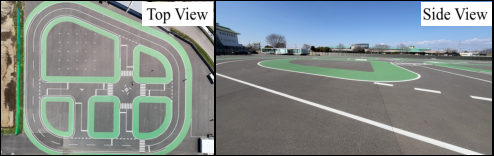
\includegraphics[width=1.0\linewidth]{images/pdf/aiformula_cource.pdf}
\caption{AI-Formula course.}
\label{fig:aiformula_course}
\end{figure}

\newpage

\section{実環境での実験方法}
実環境への適用可能性を調査するため，モビリティがスタートラインから時速 6 [km/h] で経路を走行し，コースアウトせずに障害物の手前で停止できるかの挙動を確認する．
システムの概要を\Fig{fig:exp_system}に示す．事前に設定したテキストプロンプトと画像を入力として，提案手法によりBBoxとセグメンテーションマスクを生成する．生成したBBoxとセグメンテーションマスクを用いて，後述するルールベース制御器により消失点ナビゲーションおよび障害物検出・停止タスクを実行する．
実験環境の詳細は\Table{tab:env_aiformula}の通りである．テキストプロンプトには，“white line. road. red pylon.”を指定して，その内の“white line”を消失点ナビゲーション，“red pylon”を障害物検出・停止タスクに用いた．走行経路は\Fig{fig:cource}に示す通り，破線の無い白線部分を対象とし，スタートから 20 [m] 先に障害物を設置した．

\vspace{1cm}

\begin{figure}[H]
\centering
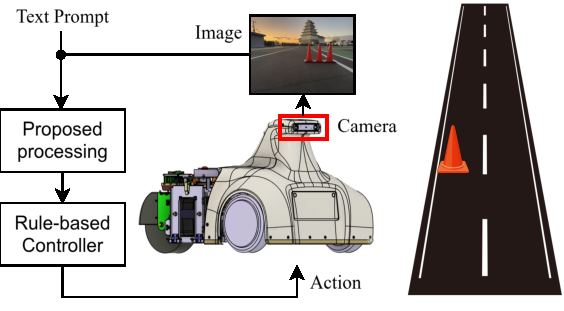
\includegraphics[width=1.0\linewidth]{images/pdf/exp_system.pdf}
\caption{Overview of the system configuration for vanishing point navigation and obstacle detection/stopping tasks.}
\label{fig:exp_system}
\end{figure}

\newpage

\vspace{1cm}

\begin{table}[H]
\centering
\caption{An experimental environment for vanishing point navigation}
\label{tab:env_aiformula}
\begin{tabular}{ll}
\hline
Computer & NVIDIA Jetson AGX Orin 32GB \\
Middleware & ROS 2 Humble \\
Input Image & 480x300 \\
Input Text & ``white line. road. red pylon.'' \\
Grounding DINO & grounding-dino-base \\
SAM Model & sam2.1\_hiera\_small \\
\hline
\end{tabular}
\end{table}

\vspace{1cm}

\begin{figure}[H]
\centering
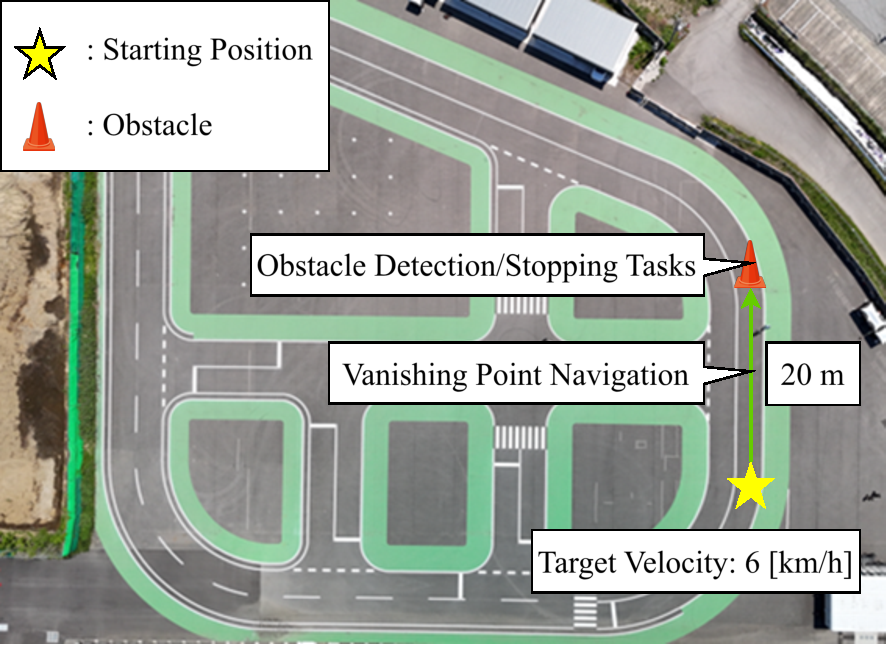
\includegraphics[width=1.0\linewidth]{images/pdf/cource.pdf}
\caption{Course and obstacle used in the experiment. (source: \cite{lang_sam_tracker})}
\label{fig:cource}
\end{figure}

\newpage

\subsection{消失点ナビゲーション}
提案手法によるセグメンテーションの結果を用いて，消失点ナビゲーションへ応用する実験を行う．ナビゲーションでは，最初に提案手法を用いてセグメンテーションされた白線を抽出する．次に，ハフ変換により2本の白線を求め，その消失点を算出する．最後に，算出した消失点が画像中心に位置するよう，PID制御に基づきモビリティのヨー角速度を制御することで白線の消失点に向かって進むようにする．これによって，モビリティはレーンの白線に沿って経路を走行する．本手順による処理結果を\Fig{fig:target}に示す．図中では，ハフ変換の出力を青線で，消失点を赤点で示している．

\vspace{1cm}

\begin{figure}[H]
\centering
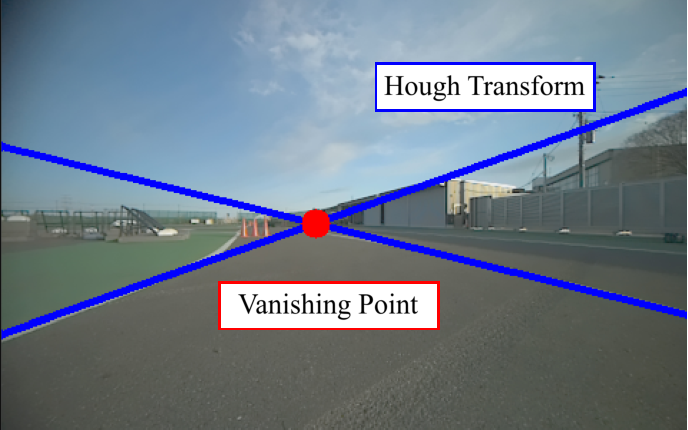
\includegraphics[width=1.0\linewidth]{images/pdf/navigation.pdf}
\caption{An example of calculating the vanishing point. (source: \cite{lang_sam_tracker})}
\label{fig:target}
\end{figure}

\newpage

\subsection{障害物検出・停止タスク}
提案手法による物体検出および物体追跡の結果を用いて，障害物検出・停止タスクへ応用する実験を行う．実験では，\Fig{fig:bbox}の赤いパイロンを障害物とする．モビリティがパイロンに接近し，検出したBBoxの面積が事前に設定したしきい値を超えた場合に自動停止させる．しきい値は，実験開始前にモビリティの5m手前にパイロンを置き，そのときに検出されるBBoxの面積を計測して設定した．

\vspace{1cm}

\begin{figure}[H]
\centering
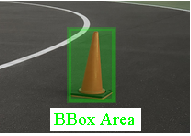
\includegraphics[width=1.0\linewidth]{images/pdf/obstacle.pdf}
\caption{Obstacle detection using the BBox area as a threshold. (source: \cite{lang_sam_tracker})}
\label{fig:bbox}
\end{figure}

\newpage

\section{実環境での実験結果}
本実験では，時速6 [km/h]で走行する自律走行モビリティを用いて，消失点ナビゲーションおよび障害物検出・停止タスクを実環境で行い，その適用可能性を調査した．その結果，モビリティは指定コースを逸脱することなく走行し，障害物手前で停止した．つまり，一例ではあるが，提案手法により事前学習なく環境を認識してコースを走行・停止できることを確認した．以下に，各タスクにおけるモビリティの挙動を詳述する．

% \newpage

\Fig{fig:follow}に，GNSSデータに基づき作成したモビリティの走行軌跡を示す．指定した約20mのコースを逸脱することなく，一定速度で走行することを確認した．ただし，部分的に蛇行する挙動も見られた．これは，システムの処理負荷増大による制御周波数の低下が原因と考えられる．認識処理のみでは2.15 FPSであった処理速度が，消失点ナビゲーションなどを含むシステム全体では低下したため，この処理遅延が蛇行につながったおそれがある．

\begin{figure}[H]
\centering
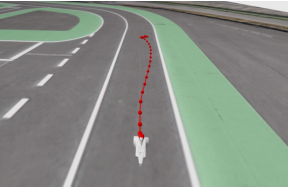
\includegraphics[width=0.9\linewidth]{images/pdf/trajectory.pdf}
\caption{The trajectory of mobility. (source: \cite{lang_sam_tracker})}
\label{fig:follow}
\end{figure}

\newpage

\Fig{fig:stop}に，障害物検出・停止タスクの結果を示す．事前に設定した目標停止距離5 [m]に対し，モビリティは障害物の約3.4 [m]手前で停止し，目標と1.6 [m]の誤差が生じた．これは，モビリティの制動距離に加え，システム全体の処理遅延も影響していると考えられる．

\vspace{1cm}

\begin{figure}[H]
\centering
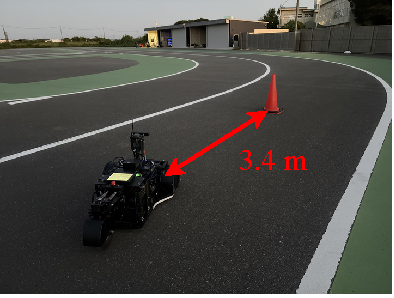
\includegraphics[width=1.0\linewidth]{images/pdf/distance.pdf}
\caption{Result of obstacle detection and stop. (source: \cite{lang_sam_tracker})}
\label{fig:stop}
\end{figure}
\newpage
